%4章提案
\section{既存手法の問題点}
既存の監視手法として次のような手法がある。
\begin{itemize}
\item 監視サーバからの問い合わせによる監視\\
	Ping,SNMPによる問い合わせ等がこの手法にあたる。
\item 機器からの通知に基づく監視\\
	SNMPTrapによる通知がこの手法である。
\end{itemize}

監視サーバからの問い合わせによる監視をIoTサービスに適応した場合、次のような問題がある。
\begin{itemize}
\item IoT機器が接続するネットワークが、プライベートアドレスを使用している場合がある\\
	IoT機器が接続するネットワークがプライベートアドレスである場合、監視サーバから問い合わせを行うことができず、監視することができない。
\item IoT機器が接続するネットワークにセキュリティの設定が施されている場合がある\\
	特に、インターネットからの特定ポートに対するアクセスをブロックしている場合がある。
	この場合も、監視サーバからの問い合わせを行うことが出来ないため、監視することが出来ない。
\item IoT機器が移動する場合がある\\
	IoT機器は移動する物に取り付けられる場合がある。
	この場合、IoT機器が接続するネットワークが頻繁にかわるため、監視サーバが問い合わせを行う宛先を頻繁に更新しなければならない。
	また、複数の機器が移動を繰り返す中で、監視サーバとのやり取りに混乱が生じる。
\end{itemize}
このため、監視サーバからの問い合わせによる監視は用いることができない。

一方、機器からの通知では、これら問題を解決する事ができる。
しかし、各IoT機器に対し個別のIDを設定する必要が有り、IoT機器が大量であることから大きな負担となる。
また、どちらの手法を取るにしても、機器監視サーバへの登録作業は行う必要が有り、負担となる。

\section{IoT機器監視・管理サービスの提案}
前章で述べたように、IoTサービスの円滑な提供の為には、IoTサービスの構造を維持する必要が有り、そのために、IoT機器を監視する必要がある。
IoT機が接続するネットワークが、プライベートアドレスを利用している等、多様であることから、機器からの通知による監視手法を取る必要がある。
しかし、IoTサービスにおいて、IoT機器は多量に使用されることや、頻繁な交換・追加がありうることから、
IoT機器へ個別の設定をすること、監視サーバへIoT機器を登録することが大きな負担となっている。

そこで私は、これら負担はIoT機器と監視サーバに設定が分散していることが原因と考え、設定を監視サーバにて一元的に管理し、IoT機器への設定を省力化する事を提案し、サービスを開発する。
このサービスの利用者は、提案するサービスから、機器追加用のトークンを受け取り、各IoT機器に対して同一のトークンを設定し、提供するプログラムを作動させる。
提供するプログラムは、監視サーバに対して、このトークンを送信し、返答として個別のIDを受け取り、自身に設定する。
サーバでは、トークンの有効性を検証し、機器の追加を自動的に行う。
図\ref{fig:prop_diag}は、提案するサービスの構成図である。
\begin{figure}[htbp]
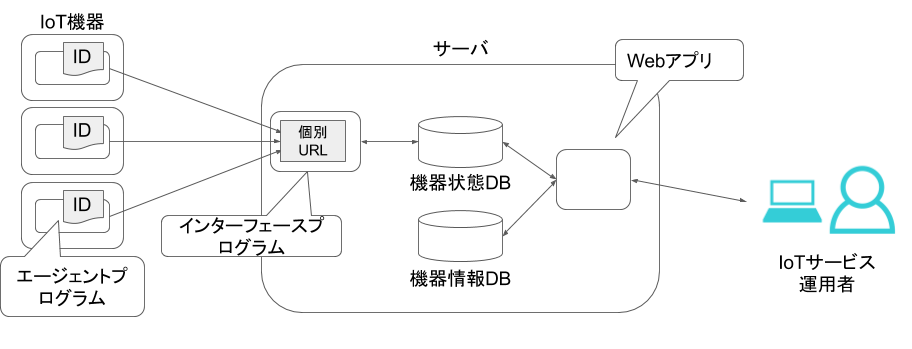
\includegraphics[width=16cm]{images/prop_diag.png}
\caption{サービス構成図}
\label{fig:prop_diag}
\end{figure}

プログラムを作動させた順に、登録された事を確認し、機器に対してIDの貼り付け等を行う。
また、IoT機器上で動作する提供プログラムは、定期的に監視サーバに対しネットワークの状態や稼働状況等を報告することで、監視を行う。

これにより、監視サーバへ各IoT機器を登録する負担と、IoT機器へ個別の設定を行うことを省力化する。
さらに、通知型でhttpsを用いた通信により、ネットワークの多様性に対応する。
また、サービスとして提供することで、従来では不可欠であった監視サーバの構築作業の負担も解決することができる。

\begin{comment}

IoT機器からの通知に基づいた、設定不要の独立した状態監視のためのサービスを提案する。
機器から通知を送ることで、IoT機器の接続されるネットワークが、プライベートアドレスを使用していても監視可能であること、ネットワークが違っていても一つの画面で確認できることを満たす。
また、状態監視の為のサービスを独立させることで、IoTサービスの変更が不要であることや、監視サーバを立てる必要が無いことを満たす。
IoT機器への設定の必要性については、あらかじめ、IoT機器自体に存在する識別IDを用いることとする。
こうすることで、監視サーバに対して、設定をする必要がなくなる。



このように、今後使用するIoT機器が増えていくことを考えると、現状の手動での監視は負担となる。
そこで、新規にIoT機器の監視に汎用的に使用できるシステムを開発し、サービスとして提供することで、問題の解決が図れるのではないかと考えた。
実験と聞き取りから得られた要件を以下にまとめる。
\begin{itemize}
\item 機器が起動し動作していることが確認できること
\item CPUの温度等も確認できると良い
\item 各機器に対する監視に関わる設定の簡略化もできたら良い
\item 機器の異常をメールなどで知らせることができたら良い
\item 機器の状態をIoTサービスごとに管理したい
\end{itemize}
\end{comment}

